\documentclass[11pt,a4paper]{memoir}

\usepackage{graphicx}
\usepackage{geometry}
\usepackage{float}
\usepackage{hyperref}
\hypersetup{
	colorlinks=true,
	linkcolor=black,
	urlcolor=blue
}

\graphicspath{{figures/}}

\renewcommand*{\maketitle}%
{
	\newgeometry{left=2cm,right=2cm,top=3cm,bottom=3.5cm}

	\begin{center}
		\begingroup
		{\Huge\textbf{POLITECNICO DI TORINO}}\\[\baselineskip]
		\rule{\textwidth}{2pt}\par
		\vspace*{1em}
		{\LARGE\textbf{Master's Degree in Computer Engineering}}\\[\baselineskip]
		\vspace*{1em}
		{\Large\textbf{Master's Degree Thesis}}\\
		\vspace*{2cm}
		{\huge\textbf{Acceleration by Separate-Process Cache for
		Memory-Intensive Algorithms on FPGA via High-Level Synthesis}}\\
		\vspace*{1cm}
		
\includegraphics[width=.3\textwidth]{figures/polito-logo}
	\end{center}
	\vfill
	\begin{minipage}{0.4\textwidth}
		\begin{flushleft}
			{\Large
				\textbf{Supervisor}\\
				Prof. Luciano Lavagno
			}
		\end{flushleft}
	\end{minipage}
	\begin{minipage}{0.4\textwidth}
		\begin{flushright} 
			{\Large
				\textbf{Candidate}\\
				Giovanni Brignone\\
				ID: 274148
			}
		\end{flushright}
	\end{minipage}  
	\vspace*{2cm}
	\begin{center}
		{\Large\textbf{Academic year 2020-2021}}
	\end{center}
	\endgroup

	\restoregeometry 
}

\begin{document}
\pagestyle{empty}
\maketitle

\frontmatter
\chapter*{Abstract}
The end of the Moore's Law validity is making the performance advance of
software run on general purpose processors more challenging than ever.
Since current technology cannot scale anymore it is necessary to approach the
problem from a different point of view: application-specific hardware can
provide higher performance and lower power consumption, while requiring higher
design efforts and higher deployment costs.

High-Level Synthesis is aimed at reducing design efforts, shrinking the gap
between hardware and software design.

FPGAs allow to reduce deployment costs, making possible to implement
special-purpose hardware modules on general-purpose underlying architecture.

FPGAs memory system is composed of three main kind of resources: registers,
Block-RAMs and external DRAMs.
Current HLS tools allow to exploit this memory hierarchy manually, in a
scratchpad-like fashion: the objective of this thesis work is to automate the
memory management by providing a easily integrable and fully customizable cache
system for High-Level Synthesis.

\pagebreak
\tableofcontents*

\mainmatter
\chapter{Background}
\section{Cache memory}
Memory devices are usually the performance bottleneck in the execution of
memory-bound algorithms.
The ideal memory should be fast, large and cheap, but current technology forces
the designer to choose a trade-off between the metrics.

A common solution to this problem is to setup a memory hierarchy in
which fast but small memories are paired with large but slow memories, which
allows to get good performance on average while containing costs.

This hierarchy can be managed by two main approaches:
\begin{itemize}
	\item \emph{Scratchpad}: different memories belongs to different addressing
		spaces: the user is in charge of manually choosing what memory
		to access: this approach allows to optimally exploit the
		hierarchy at the cost of high design effort.
	\item \emph{Cache}: different memories belongs to the same addressing
		space: the system automatically uses the whole hierarchy
		exploiting spatial locality (accessed data is likely physically
		close to previously accessed data) and temporal locality
		(accessed data has likely recently been accessed), which are
		typical of many algorithms.
\end{itemize}

\subsection{Structure}
A cache memory is logically split into \emph{sets} containing \emph{lines} (or
\emph{ways}) which are in turn made up of \emph{words}, as shown in
Figure~\ref{fig:cache_logic_structure}.

\begin{figure}
	\centering
	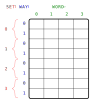
\includegraphics[width=.5\textwidth]{cache_logic_structure}
	\caption{Cache logic structure.}
	\label{fig:cache_logic_structure}
\end{figure}

Whenever a word $w$ is requested there are two possibilities:
\begin{itemize}
	\item \emph{Hit}: $w$ is present in the cache: the request can be
		immediately fulfilled.
	\item \emph{Miss}: $w$ is not present in the cache: it is necessary to
		retrieve it from lower level memory before fulfilling the request.
\end{itemize}
During the data retrieving a cache line is filled with a block of contiguous
words loaded from the lower level memory, trying to exploit spatial locality of
future accesses, while mapping policies and replacement policies determine which
cache line to overwrite, trying to exploit temporal locality.

If the cache memory is writable, data consistency is ensured by a consistency policy.
\subsection{Policies}
\subsubsection{Mapping policy}
The mapping policy is in charge of statically associating a lower level memory
line to a cache set.

The \emph{set associative} policy is the most common mapping policy: given a
cache memory with $s$ sets of $w$ words, the word address (referred to the lower
level memory) bits are split into three parts (as shown in
Figure~\ref{fig:address_partitioning}):
\begin{enumerate}
	\item $\log_2(w)$: offset of the word in the line.
	\item $\log_2(s)$: set.
	\item remaining MSBs: tag identifying the specific line.
\end{enumerate}

\begin{figure}
	\centering
	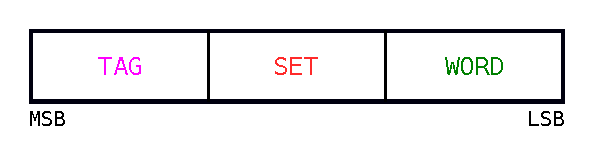
\includegraphics[width=.5\textwidth]{address_partitioning}
	\caption{Set associative policy address bits meaning.}
	\label{fig:address_partitioning}
\end{figure}

Special cases of this policy are:
\begin{itemize}
	\item \emph{Direct mapped} policy: each set is composed of a single line:
		the set bits identify a specific cache line, therefore there is
		no need for a replacement policy.
	\item \emph{Fully associative} policy: there is only a single set,
		therefore the line is fully determined by the replacement policy.
\end{itemize}

\subsubsection{Replacement policy}
The replacement policy is in charge of dynamically associating a lower level
memory line to a cache line of a set.

Multiple solutions of this problem have been developed, trying to maximize
the temporal locality exploitation.
Among the most commonly used solutions there are:
\begin{itemize}
	\item \emph{First-In First-Out}: the line to be replaced is the first
		one that has been inserted to the cache.
	\item \emph{Least recently used}: the line to be replaced is the one
		that has least recently been accessed.
\end{itemize}

\subsubsection{Consistency policy}
The consistency policy is in charge of ensuring data consistency between memories
belonging to different hierarchy levels.

The most common solutions to this problem are:
\begin{itemize}
	\item \emph{Write-back}: write accesses are performed to the highest
		level memory and lower level memories are updated when the cache
		line is replaced only.
	\item \emph{Write-through}: each write access is propagated along the
		whole hierarchy.
\end{itemize}

\section{High-Level Synthesis}
The High-Level Synthesis (HLS) is an Electronic Design Automation technique
aimed at translating an algorithm description in an high-level software
programming language (such as C and C++) into an Hardware Description Language
(HDL) description.

HLS allows to design more complex systems in less time, compared to HDL design,
moreover makes the hardware and software co-design much easier, at the cost of
less expressiveness.

\subsection{Workflow}
The typical HLS workflow consists in:
\begin{enumerate}
	\item software implementation: the top level entity is a C function:
		the function arguments are the entity ports and the functionality
		is implemented in SW; in order to guarantee synthesizability
		some constraints should be respected (e.g. no dynamic memory
		allocation).
	\item software verification: the testbench can be developed as a simple
		main function which calls the top level entity function,
		therefore the functionality is verified like any SW:
		it is possible to exploit traditional tools (e.g. debuggers,
		print statements...).
	\item hardware synthesis: the synthesizer generates an RTL description
		of the top level entity. It is possible to generate different
		architectures by setting up some parameters through dedicated
		directives.
	\item hardware verification: the RTL description is simulated, to make
		sure that SW and HW outputs match.
\end{enumerate}

\subsection{Optimization techniques}
Typical optimization techniques used by HLS for improving performance include:
\begin{itemize}
	\item pipelining: loops and functions logic can be pipelined so that
		successive iterations/calls can start while previous ones are
		still running. The introduced parallelism allows to increase
		the throughput at a limited additional area cost (only pipeline
		registers and an FSM are required).
	\item dataflow: different functions composing the design are called in
		a pipelined fashion (similarly to pipelining, but at task level,
		instead of instruction level).
	\item loop unrolling: the loop logic is instantiated multiple times,
		to execute multiple loop iterations in parallel, reducing latency
		and improving throughput.
	\item memory optimizations
		\begin{itemize}
			\item bursting: multiple memory accesses are aggregated
				to reduce overall latency and improving throughput.
			\item interface widening: multiple data elements are
				packed into a single bigger word, to perform
				multiple accesses at the same time.
		\end{itemize}
\end{itemize}

\section{FPGAs}
Field Programmable Gate Arrays are integrated circuits able to implement special
purpose circuits described in HDL, thanks to their programmable logic blocks and
interconnections.
\subsection{Memory system}
An FPGA memory system is typically made up of:
\begin{itemize}
	\item registers: the fastest but most expensive memories, therefore
		there are only a few.
	\item block RAMs: on chip RAMs accessible through simple and fast
		interface.
	\item external DRAM: off chip RAMs through complex and slow interface
		(e.g. AXI).
\end{itemize}

\section{Previous work}

\chapter{Architecture}
\section{Basic architecture}
The fundamental idea behind the proposed architecture is to keep application and
cache logic into separate processes, in order to simplify synthesizer job and
possibly obtain a better performing circuit, as shown in Figure~\ref{fig:basic_arch}.

When application needs to access memory:
\begin{enumerate}
	\item application writes the request to the request FIFO.
	\item cache reads the request FIFO and checks if it causes a miss
	\item in case of miss, cache issues a request to the AXI interface to
		prepare its own memory for fulfilling the requested access.
	\item cache performs the access to its own memory and writes the outcome
		to the response FIFO (in case of a read request).
\end{enumerate}

\begin{figure}
	\centering
	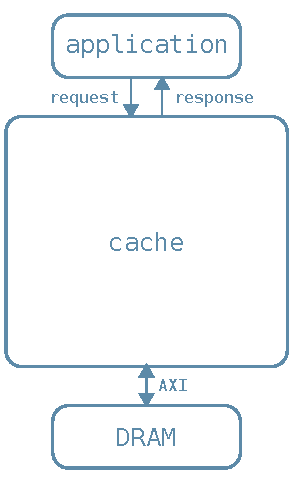
\includegraphics[width=.3\textwidth]{basic_arch}
	\caption{Outer view of the basic architecture of a kernel using the cache.}
	\label{fig:basic_arch}
\end{figure}

\subsection{Single-process solution}
The straightforward solution is to design the cache as a single process, but
the synthesizer would generate a pipeline which includes the AXI interfacing and
any request, no matter if it is an hit, has to pass through it, cancelling any
performance advantage from the cache.

\subsection{Multi-process solution}
The desirable cache architecture should be made up of a short pipeline which
runs at full speed in case of hit and stalls in case of miss.
To make the synthesizer generate such an architecture, the cache have been split
into two processes (Figure~\ref{fig:basic_arch_inner}):
\begin{itemize}
	\item core: it is in charge of managing communication with application
		and keeping cache data structures up to date.
	\item memory interface: it is in charge of interfacing with the AXI
		interface.
\end{itemize}

This solution makes the core pipeline shorter since it does not have to deal
with AXI interfacing and in case of miss the pipeline stalls thanks to the
blocking read of the memory interface response.

\begin{figure}
	\centering
	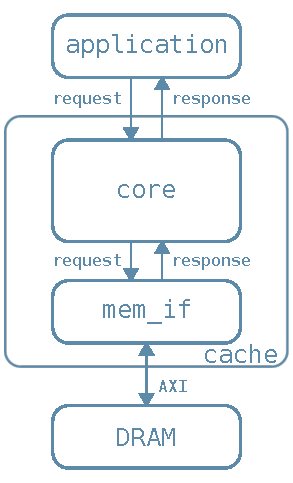
\includegraphics[width=.3\textwidth]{basic_arch_inner}
	\caption{Inner view of the basic architecture of a kernel using the cache.}
	\label{fig:basic_arch_inner}
\end{figure}

\section{Optimizations}
\subsection{L1 cache}
\subsection{Multiple read ports}

\chapter{Implementation}
\section{Multi-process modeling}
\subsubsection{Process modeling}
\subsubsection{Communication modeling}
\section{RAW dependencies}

\chapter{Results}
\chapter{Conclusion}

\end{document}

